\documentclass[a4paper]{article}
\usepackage{better_poster}
\usepackage[compact]{titlesec}
\titlespacing{\section}{0pt}{2ex}{1ex}
\titlespacing{\subsection}{0pt}{1ex}{0ex}
\linespread{0.92}


% ---- fill in from here

% authors
\title{RingTMP: A Communication Optimised Distributed Neural Network}
\author{Chris Hopkins}

% type of poster: [exp]erimental results, [methods], [theory]
% Disclaimer: the original classification had "study" and "intervention" as separate categories. I group them under experimental results.
\newcommand\postertype{exp} % [exp],[methods],[theory]

\begin{document}

% main point of your study
\makefinding{
\textbf{Novel paradigm reduces communication} within distributed neural network \textbf{as much as 8x}.
}

% \textbf{Reducing communication} within distributed neural networks as much as \textbf{8x} to \textbf{improve scalability}.  

% the main text of your poster goes here
\makemain{
    % you can have 1 or 2 columns
    \raggedcolumns
    \begin{multicols}{2}
        \section{Intro}
        \begin{compactitem}
            \item Current distributed machine learning (DML) models are reaching
            the limits of scalability due to increase communication leading to
            network saturation, ultimately limiting training speed.
            \item Using a new paradigm to distribute nodes could result in less
            communication therefore more scalability \& reduced training times.
        \end{compactitem}
        
        \section{Problem Description}
        \begin{compactitem}
            \item Neural networks function by using using parameters in each
            layer to transform the input, and pass the activation to then next
            layer.
            \item The parameter server (a popular DML paradigm) functions
            by broadcasting all parameters to its workers, which reply with a
            modified version of those parameters.
            \item Can we decrease communication by passing activations rather
            than parameters, would this affect training?
        \end{compactitem}
        \columnbreak

        \section{Results}
        
        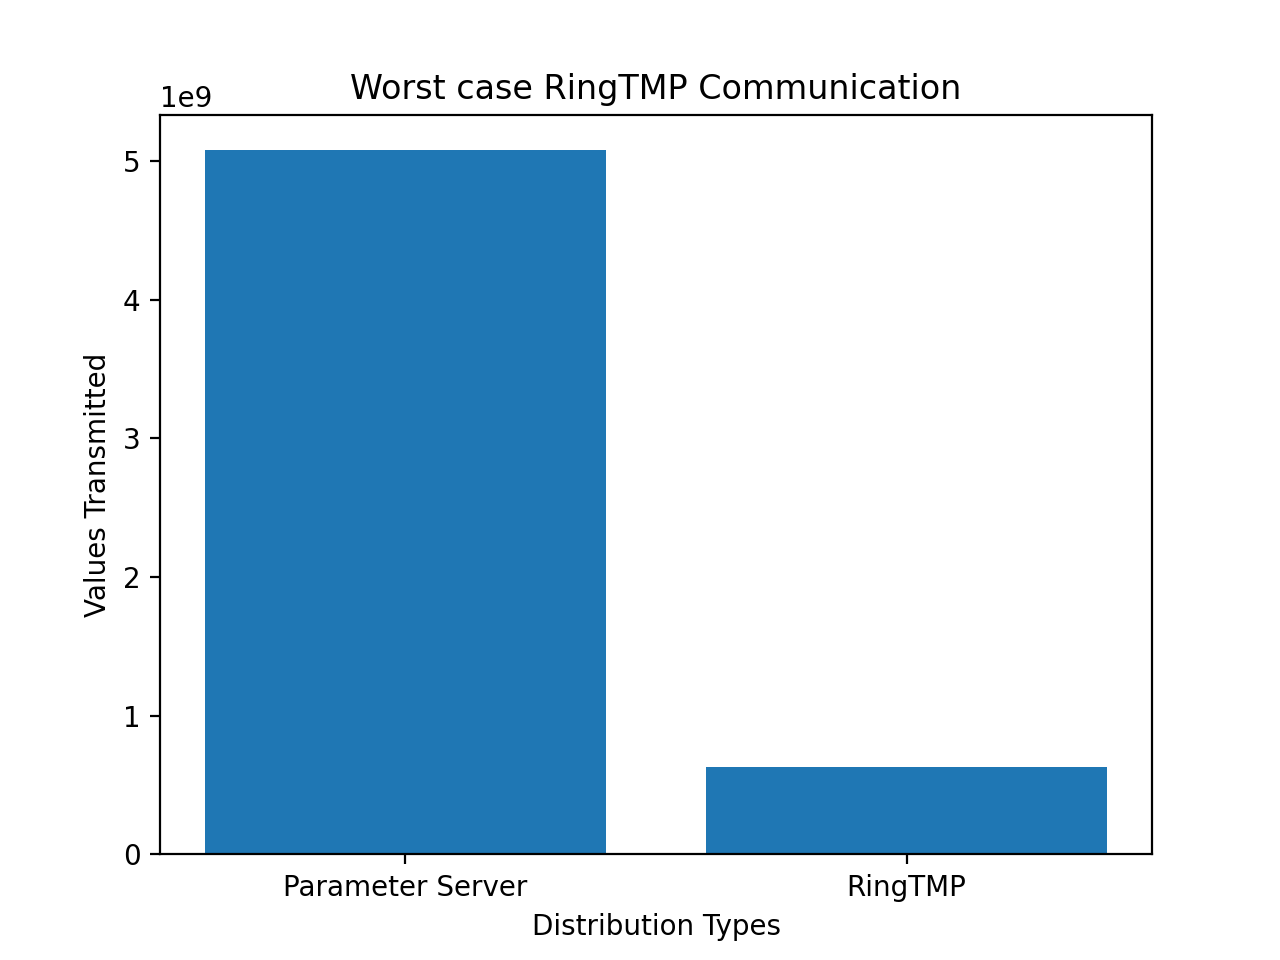
\includegraphics[width=0.9\linewidth]{worst_case_communication}\newline
        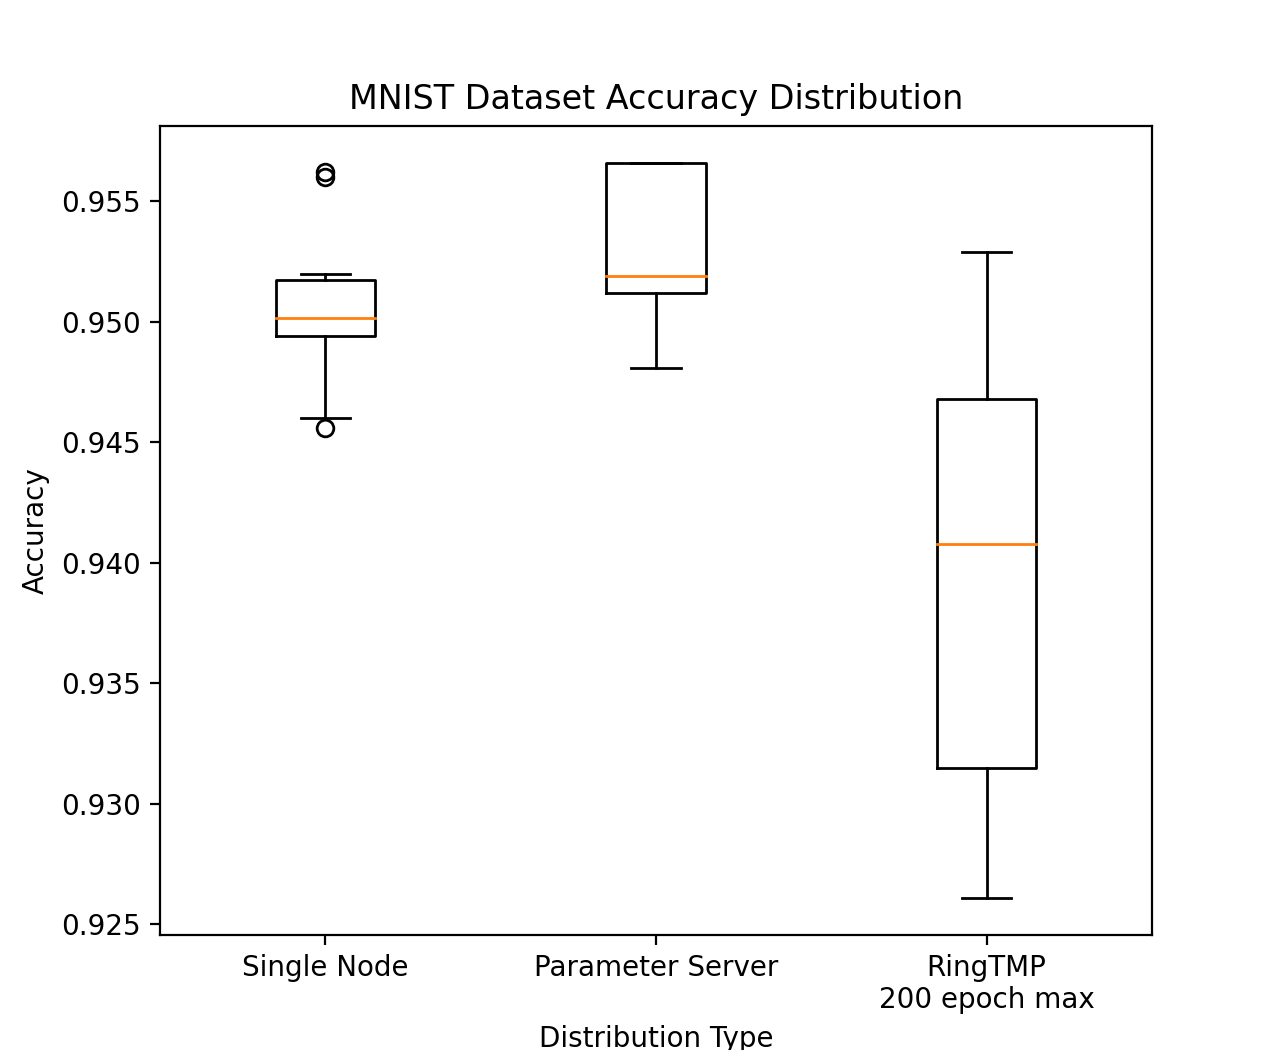
\includegraphics[width=0.9\linewidth]{mnist_accuracy_200}
        \begin{compactitem}
            \item We trained a single node, a parameter server and a RingTMP
            implementation on the Iris and MNIST numbers dataset (10, 5 times
            respectively)
            \item We found while RingTMP produced slightly less accurate models,
            but reduces communication 8x per unit time even in the worst case.
        \end{compactitem}
    
    \end{multicols}
}
% If you have extra figures or data to show
\makeextracolumn{
    \begin{center}
        RingTMP
    \end{center}
    \begin{center}
        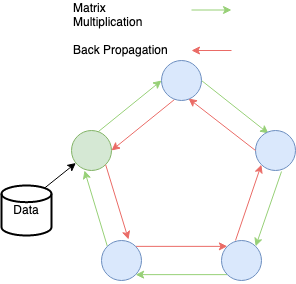
\includegraphics[width=0.65\linewidth]{ringtmp_example}
    \end{center}
    \begin{center}
        Parameter Server
    \end{center}
    \begin{center}
        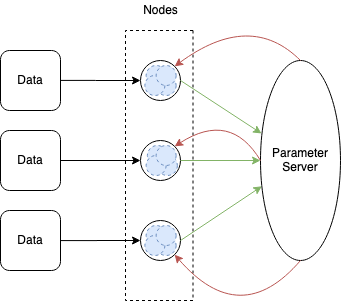
\includegraphics[width=0.65\linewidth]{parameter_server}
    \end{center}
    \begin{center}
        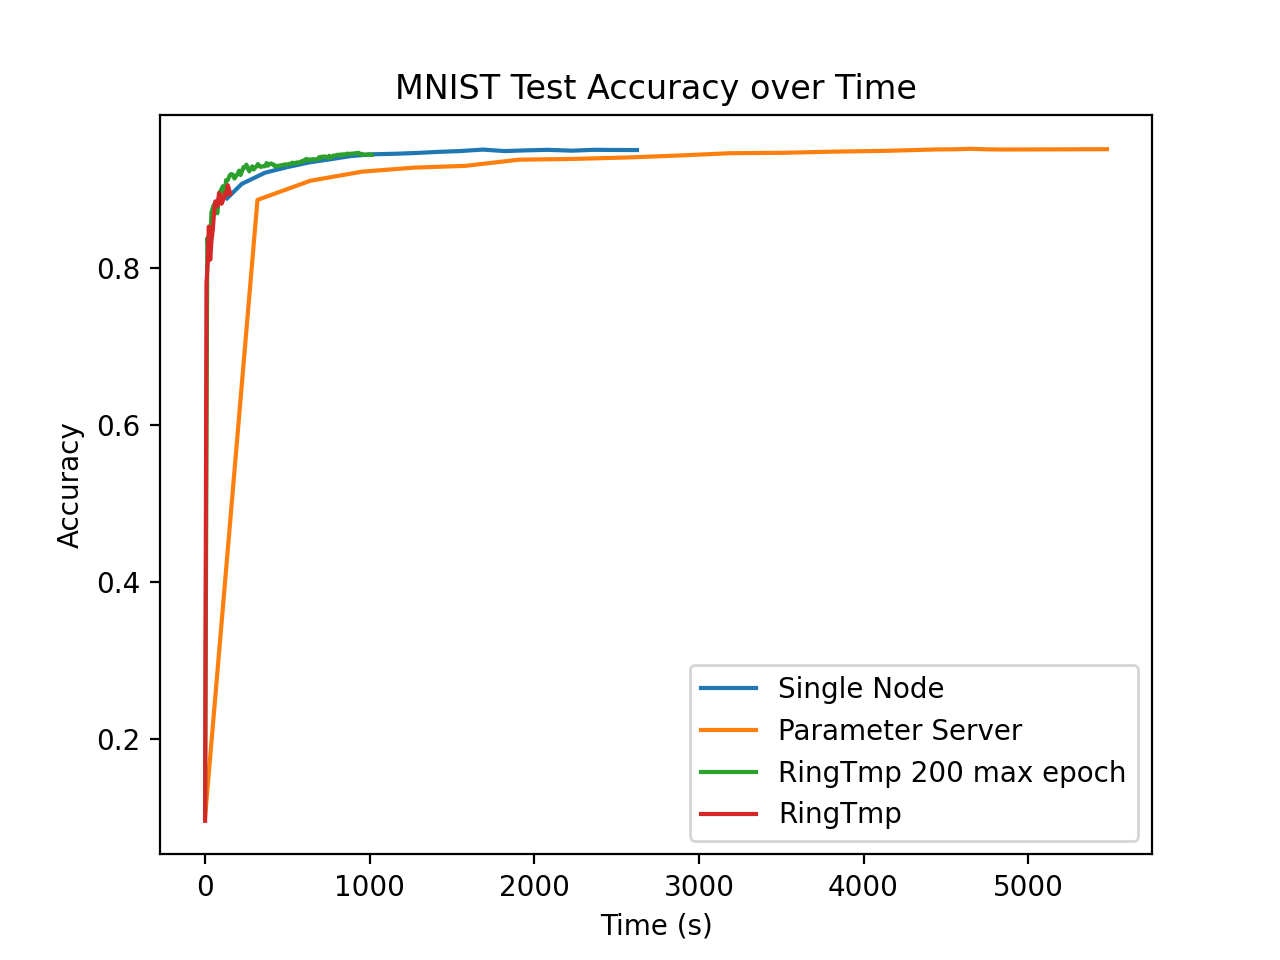
\includegraphics[width=0.9\linewidth]{mnist_accuracy_over_time}
        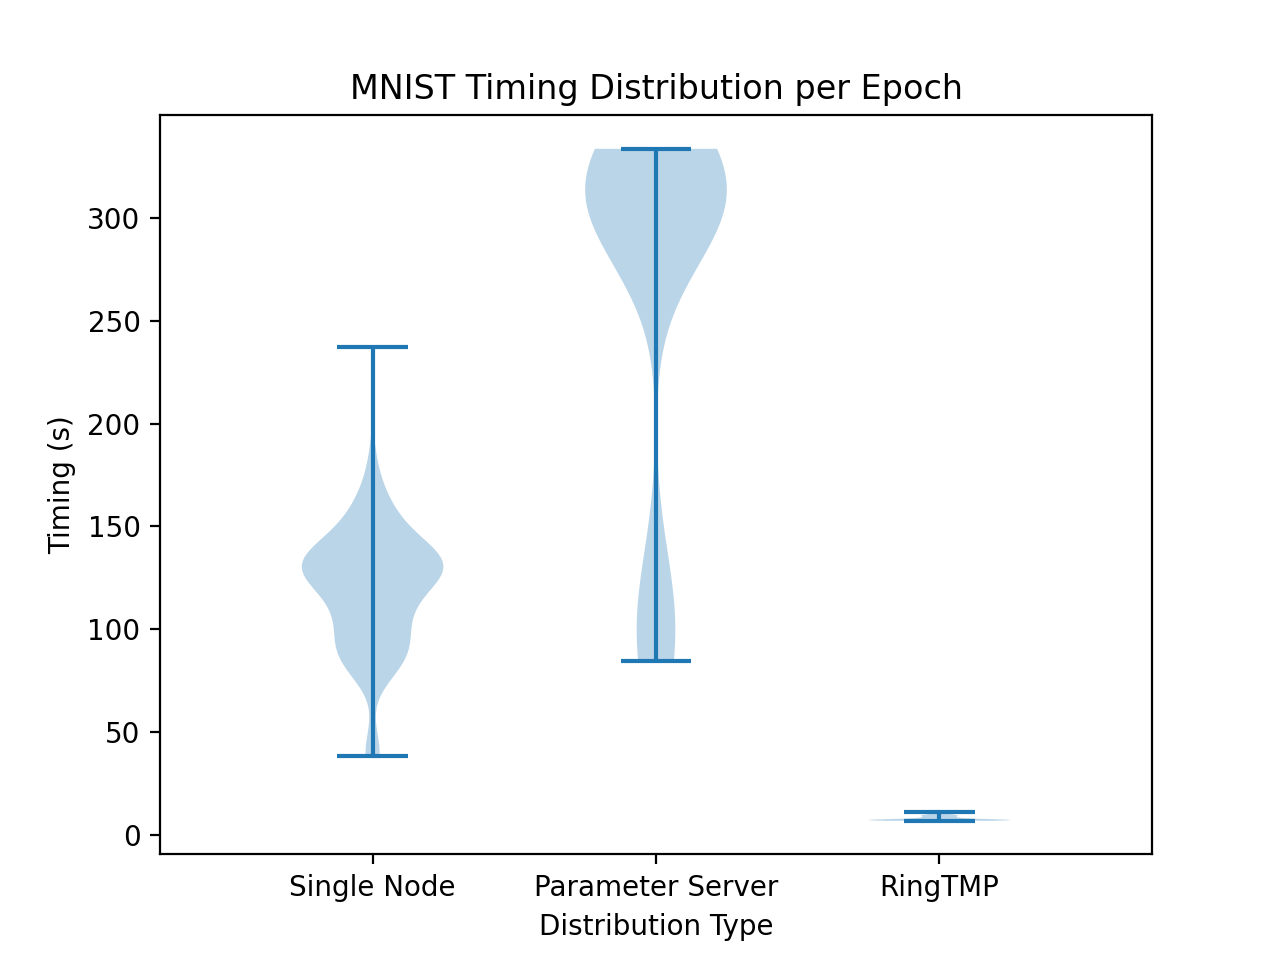
\includegraphics[width=0.9\linewidth]{images/mnist_timing_violinplot}
    \end{center}
    
    
    % \begin{itemize}
    % \setlength\itemsep{0.1em}
    %     \item Stuff you don't want to forget
    %     \item But is not essential
    % \end{itemize}
}

% footer
% generate qr code from https://www.qr-code-generator.com/ and replace qr_code.png
% default: barcode on the left
\makefooter{images/blue_swansea_logo}{images/project_qr_code}

% replace with this like for barcode on the right
%\makealtfooter{images/uni_logo.png}{images/qr-code.png}
 
\end{document}